\documentclass[a4paper,11pt]{article}

%%%%%%%%%%%%%%%%%%%%%%%%%%%%%%%%%%%%%%%%%%%%%%%%%%%%%%%%%%%%%%%%%%%%%%%%
% Paquetes utilizados
%%%%%%%%%%%%%%%%%%%%%%%%%%%%%%%%%%%%%%%%%%%%%%%%%%%%%%%%%%%%%%%%%%%%%%%%

% Graficos complejos
\usepackage{graphicx}
\usepackage{caption}
\usepackage{subcaption}
\usepackage{placeins}

% Soporte para el lenguaje español
\usepackage{textcomp}
\usepackage[utf8]{inputenc}
\usepackage[T1]{fontenc}
\DeclareUnicodeCharacter{B0}{\textdegree}
\usepackage[spanish]{babel}

% Matematicos
\usepackage{amssymb,amsmath}

% Soporte para arrays y tabs y formatos de columna
\usepackage{array}

% Soporte para subrayado
\usepackage{ulem}

% Soporte para enumerados
\usepackage{enumerate}

% PDFs embebidos para el apendice
\usepackage{pdfpages}

% Soporte para warnings
\usepackage{fixltx2e}

% Soporte para headers y footers
\usepackage{fancyhdr}
\renewcommand{\headrulewidth}{0pt}
\renewcommand{\footrulewidth}{0pt}
\usepackage{color}

\definecolor{color01}{rgb}{0.40,0.40,0.40}

\newcommand{\tab}{\hspace{5mm}}

% Formato de parrafo
\setlength{\parskip}{1ex plus 0.5ex minus 0.2ex}

%%%%%%%%%%%%%%%%%%%%%%%%%%%%%%%%%%%%%%%%%%%%%%%%%%%%%%%%%%%%%%%%%%%%%%%%
% Titulo
%%%%%%%%%%%%%%%%%%%%%%%%%%%%%%%%%%%%%%%%%%%%%%%%%%%%%%%%%%%%%%%%%%%%%%%%

% Titulo principal del documento.
\title{\textbf{Trabajo Práctico 1: Colas}}

% Informacion sobre los autores.
\author{\\
  Cesar Buffevant, \textit{P. ??.???}                              \\
  \texttt{buffevant@gmail.com}                                     \\ [2.5ex]
  Juan Pecora, \textit{P. ??.???}                                  \\
  \texttt{jlopezpecora@gmail.com}                                  \\ [2.5ex]
  Flavio Olivieri, \textit{P. ??.???}                              \\
  \texttt{flavio.olivieri@gmail.com}                               \\ [2.5ex]
  Sergio Matias Piano, \textit{P. 85.191}                          \\
  \texttt{smpiano@gmail.com}                                       \\ [2.5ex]
  Florencia Tristant, \textit{P. ??.???}                           \\
  \texttt{flotristant@gmail.com}                                   \\ [2.5ex]
                                                                   \\
  \normalsize{1er. Cuatrimestre de 2015}                           \\
  \normalsize{71.15 Modelos y Optimización 2}                      \\
  \normalsize{Facultad de Ingeniería, Universidad de Buenos Aires} \\
}
\date{}

%%%%%%%%%%%%%%%%%%%%%%%%%%%%%%%%%%%%%%%%%%%%%%%%%%%%%%%%%%%%%%%%%%%%%%%%
% Documento
%%%%%%%%%%%%%%%%%%%%%%%%%%%%%%%%%%%%%%%%%%%%%%%%%%%%%%%%%%%%%%%%%%%%%%%%
\begin{document}
\thispagestyle{empty}
\maketitle

\clearpage

\vspace{8pt}
\section*{\textbf{Ejercicio 1}}

\baselineskip=13pt
En una sastrería hay una sección de arreglo y reforma de la ropa vendida a sus 
clientes, que es atendida por un sastre. El número de clientes que requieren arreglos 
arriban a dicha sección con una distribución de Poisson con una media de 24 clientes 
por hora. Debido a que el servicio es gratuito, todos los clientes están dispuestos 
a esperar el tiempo que sea necesario para poder utilizarlo. El tiempo de atención 
es en promedio de 2 minutos por cliente, siendo exponencial la distribución de 
los tiempos de servicio. Calcular:

\leftskip=36pt
\parindent=-18pt
\begin{enumerate}[a.]
  \item ¿Cual es en promedio, el número de clientes en la sección?

  \item ¿Cuánto tiempo permanece, en promedio, un cliente en la sección?

  \item ¿Cual es la probabilidad de que el sastre esté desocupado?

  \item ¿Cual es en promedio, el número de clientes que están esperando recibir 
  el servicio?
\end{enumerate}

\vspace{13pt}
\leftskip=0pt
\parindent=0pt
\subsection*{\textbf{Resolución}}

Como sistema se entiende toda la sección de arreglo y reforma.\label{h.ucd2riukxd97}

\vspace{8pt}
\subsubsection*{Hipotesis:}

Se verifican las hipótesis de un P/P/1. El enunciado dice explícitamente que 
todos los clientes están dispuestos a esperar el tiempo que sea necesario, lo 
cual se puede interpretar como una cola con capacidad infinita.

\begin{enumerate}[1.]
  \item Tipo de proceso de arribo de clientes responde a distribución Poisson.
  \item Tipo de proceso de servicio a los clientes en el sistema responde a distribución Poisson.
  \item Hay un único canal de atención.
  \item El sistema tiene capacidad infinita.
  \item La disciplina de atención es FIFO.
  \item La población es infinita.
  \item Se forma una única cola frente al canal.
  \item El sistema se encuentra en régimen estacionario.
  \item La población no presenta fenómeno de impaciencia.
\end{enumerate}

\vspace{13pt}
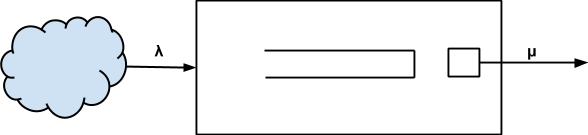
\includegraphics[width=341pt, height=101pt, keepaspectratio=true]{TP1-Colas-fig001.png}

\vspace{27pt}
Parámetros del modelo:

$\lambda = 24 [clientes/hora]$

$T_s = 2 [minutos] \frac{1[hora]}{60[minutos]} = 0.033 [horas]$ → $\mu = 30 [clientes/hora]$

\vspace{13pt}
A  El número de clientes en la sección, es decir el número de clientes en el 
sistema, es L.

$L = \frac{\lambda}{\mu - \lambda} = \frac{24}{30 - 24} = 4 clientes/hora$

%\vspace{27pt}
%B. El tiempo que permanece un cliente en la sección, es decir, en el sistema es 
%W:
%
%%%\begin{figure}[htbp]
%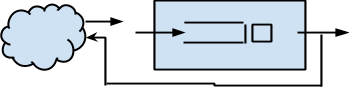
\includegraphics[width=281pt, height=27pt, keepaspectratio=true]{TP1-Colas-fig003.png}
%%%\caption{This should be the caption for \texttt{TP1-Colas-fig003.png}.}
%%%\end{figure}
%
%\vspace{27pt}
%C. La probabilidad de que el sastre esté desocupado es la probabilidad de que 
%en la sección no haya nadie, es decir P(0)
%
%%%\begin{figure}[htbp]
%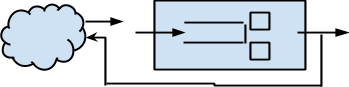
\includegraphics[width=152pt, height=25pt, keepaspectratio=true]{TP1-Colas-fig004.png}
%%%\caption{This should be the caption for \texttt{TP1-Colas-fig004.png}.}
%%%\end{figure}
%
%\vspace{13pt}
%D. El número de clientes esperando recibir el servicio son los clientes que están 
%en la cola, es decir L\textsubscript{c}.
%
%%%\begin{figure}[htbp]
%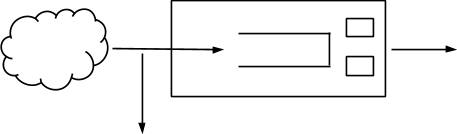
\includegraphics[width=170pt, height=29pt, keepaspectratio=true]{TP1-Colas-fig005.png}
%%%\caption{This should be the caption for \texttt{TP1-Colas-fig005.png}.}
%%%\end{figure}
%
%\label{h.k0o10jsxzae}
%
%\vspace{35pt}
%\subsubsection*{{\color{color01} \textbf{Ejercicio 2}}}
%
%Un establecimiento de reparaciones, atendido por un solo operario, recibe un promedio 
%de cuatro clientes por hora, los cuales traen pequeños aparatos para reparar. 
%El mecanico los inspecciona para encontrar defectos y muy a menudo puede arreglarlos 
%de inmediato, o de otro modo emitir un diagnostico. En promedio, todo le toma 6 
%minutos por aparato. Los arribos tienen una distribución de de Poisson y el tiempo 
%de servicio tiene una distribución exponencial. Calcular:
%
%\leftskip=36pt
%\parindent=-18pt
%A.\tab La probabilidad de que el taller esté vacío.
%
%B.\tab La probabilidad de que tres clientes estén en el taller.
%
%C.\tab La probabilidad de encontrar por lo menos un cliente en el taller.
%
%D.\tab El número promedio de clientes en el taller.
%
%E.\tab El tiempo promedio que un cliente debe permanecer en el taller.
%
%F.\tab El número promedio de clientes que esperan ser atendidos.
%
%G.\tab El tiempo promedio que un cliente debe esperar para ser atendido.
%
%\vspace{13pt}
%\leftskip=0pt
%\parindent=0pt
%Consideramos el sistema como el taller, con el operario incluido. El enunciado 
%no dice nada con respecto a la capacidad de la cola, por lo que entendemos que 
%hay suficiente lugar como para albergar a toda la gente que arribe.
%
%\vspace{13pt}
%Parámetros del modelo:
%
%$\lambda$ = 4 clientes/hora
%
%T\textsubscript{s} = 6 minutos = 0.1 horas → $\mu$ = 10 clientes/hora.
%
%\vspace{13pt}
%A La probabilidad de que el taller esté vacío es la probabilidad de que no haya 
%ningún cliente en el sistema, es decir P(0).
%
%P(0) = 1 - = 1 - 4/10 = 0.6
%
%
%\vspace{13pt}
%B. La probabilidad de que tres cliente estén en el sistema es
%
%%%\begin{figure}[htbp]
%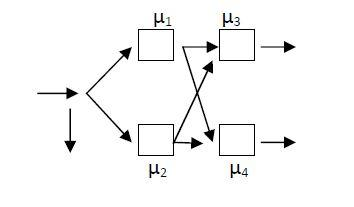
\includegraphics[width=211pt, height=17pt, keepaspectratio=true]{TP1-Colas-fig008.png}
%%%\caption{This should be the caption for \texttt{TP1-Colas-fig008.png}.}
%%%\end{figure}
%
%\vspace{27pt}
%C. La probabilidad de encontrar por lo menos a un cliente es P(n \texttt{>} 0) 
%= 1 - P(0) = 1 - 0.6 = 0.4.
%
%\vspace{13pt}
%D. El número promedio de clientes en el taller es el número promedio de clientes 
%en el sistema, es decir L.
%
%%%\begin{figure}[htbp]
%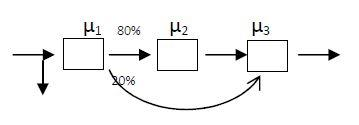
\includegraphics[width=333pt, height=27pt, keepaspectratio=true]{TP1-Colas-fig009.png}
%%%\caption{This should be the caption for \texttt{TP1-Colas-fig009.png}.}
%%%\end{figure}
%
%\vspace{27pt}
%E. El tiempo promedio que un cliente debe permanecer en el taller es el tiempo 
%que un cliente debe permanecer en el sistema, es decir W.
%
%%%\begin{figure}[htbp]
%\includegraphics[width=252pt, height=27pt, keepaspectratio=true]{TP1-Colas-fig010.png}
%%%\caption{This should be the caption for \texttt{TP1-Colas-fig010.png}.}
%%%\end{figure}
%
%\vspace{27pt}
%F. El número de clientes que esperan ser atendidos son los clientes esperando 
%en la cola, es decir L\textsubscript{c}.
%
%%%\begin{figure}[htbp]
%\includegraphics[width=332pt, height=29pt, keepaspectratio=true]{TP1-Colas-fig011.png}
%%%\caption{This should be the caption for \texttt{TP1-Colas-fig011.png}.}
%%%\end{figure}
%
%\vspace{27pt}
%G. El tiempo promedio que un cliente tiene que esperar para ser atendido es el 
%tiempo que pasa en la cola, es decir W\textsubscript{c}.
%
%%%\begin{figure}[htbp]
%\includegraphics[width=300pt, height=29pt, keepaspectratio=true]{TP1-Colas-fig012.png}
%%%\caption{This should be the caption for \texttt{TP1-Colas-fig012.png}.}
%%%\end{figure}
%
%\label{h.c9kpqzkqh5j9}
%
%\vspace{49pt}
%\subsubsection*{{\color{color01} \textbf{Ejercicio 3}}}
%
%Un banco está desarrollando la prestación de un nuevo servicio, para lo cual 
%ha habilitado una ventanilla. Como el desarrollo del mismo está basado en una 
%campaña publicitaria que hace mención al mínimo tiempo de espera que se requiere, 
%el gerente de la sucursal ha decidido encarar el estudio científico del problema 
%a fin de no exponerse a un fracaso. Hasta ahora se cuenta con los siguientes datos:
%
%\leftskip=36pt
%\parindent=-18pt
%\tab Lapso medio entre arribo de usuarios: 8 minutos (distribución exponencial)
%
%\tab Tiempo medio de atención en ventanilla: 2 minutos (distribución exponencial).
%
%\leftskip=0pt
%\parindent=0pt
%Determinar:
%
%\leftskip=36pt
%\parindent=-18pt
%A.\tab La probabilidad de esperar.
%
%B.\tab La longitud promedio de la cola.
%
%C.\tab La velocidad promedio de arribos que haría que el tiempo de espera en la 
%cola supere los 4 minutos.
%
%\vspace{13pt}
%\leftskip=0pt
%\parindent=0pt
%Consideramos el sistema como la ventanilla más la cola. El enunciado no dice nada 
%con respecto a la capacidad de la cola, por lo que entendemos que hay suficiente 
%lugar como para albergar a toda la gente que arribe.\label{h.eoq63ml893zx}
%
%\vspace{8pt}
%{\color{color01} \emph{Hipotesis:}}
%
%Se verifican las hipótesis de un P/P/1.
%
%\vspace{13pt}
%Parámetros del modelo:
%
%T = 8 minutos → $\lambda$ = 0.125 clientes/minuto.
%
%Ts = 2 minutos → $\mu$ = 0.5 clientes/minuto.
%
%\vspace{13pt}
%A. La probabilidad de esperar es la probabilidad de que en el sistema haya algún 
%cliente, es decir P(n \texttt{>} 0) = 1 - P(0).
%
%%%\begin{figure}[htbp]
%\includegraphics[width=275pt, height=25pt, keepaspectratio=true]{TP1-Colas-fig013.png}
%%%\caption{This should be the caption for \texttt{TP1-Colas-fig013.png}.}
%%%\end{figure}
%
%\vspace{27pt}
%B. La longitud promedio de la cola es la cantidad de clientes en promedio esperando 
%para ser atendidos, es decir L\textsubscript{c}.
%
%%%\begin{figure}[htbp]
%\includegraphics[width=428pt, height=31pt, keepaspectratio=true]{TP1-Colas-fig014.png}
%%%\caption{This should be the caption for \texttt{TP1-Colas-fig014.png}.}
%%%\end{figure}
%
%\vspace{27pt}
%C. El tiempo de espera en la cola es W\textsubscript{c}, es decir:
%
%\vspace{13pt}
%%%\begin{figure}[htbp]
%\includegraphics[width=321pt, height=30pt, keepaspectratio=true]{TP1-Colas-fig015.png}
%%%\caption{This should be the caption for \texttt{TP1-Colas-fig015.png}.}
%%%\end{figure}
%
%\label{h.6r62cgyud887}
%
%\vspace{35pt}
%\subsubsection*{{\color{color01} \textbf{Ejercicio 4}}}
%
%Teniendo en cuenta el ejercicio 2, considerar todas las suposiciones anteriores, 
%excepto que si hay tres clientes en el taller, cualquier otro cliente que llegue 
%se retirará.
%
%Determinar entonces:
%
%\leftskip=36pt
%\parindent=-18pt
%1.\tab La probabilidad de que el taller esté vacío.
%
%2.\tab La probabilidad de que tres clientes estén en el taller.
%
%3.\tab La probabilidad de encontrar por lo menos un cliente en el taller.
%
%4.\tab El número promedio de clientes en el taller.
%
%5.\tab El tiempo promedio que un cliente debe permanecer en el taller.
%
%6.\tab El número promedio de clientes que esperan ser atendidos.
%
%7.\tab El tiempo promedio que un cliente debe esperar para ser atendido.
%
%8.\tab La cantidad promedio de clientes que se retiran sin ser atendidos.\label{h.fut7k3oybvll}
%
%\vspace{21pt}
%\leftskip=0pt
%\parindent=0pt
%{\color{color01} \emph{Hipótesis}}
%
%\leftskip=36pt
%\parindent=-18pt
%\tab El proceso de llegada de los clientes responde a un proceso Poisson.
%
%\tab El proceso de atención de los clientes responde a un proceso Poisson.
%
%\tab La población es infinita
%
%\tab Se forma una única cola frente al canal de atención.
%
%\tab Existe un único canal de atención.
%
%\tab La capacidad del sistema es infinita
%
%\tab La atención de los clientes de la cola es FIFO
%
%\tab El sistema se encuentra en condiciones estables.
%
%\tab \emph{La población presenta el fenómeno de impaciencia.\label{h.opqdcj4n3uxj}}
%
%\vspace{21pt}
%\leftskip=0pt
%\parindent=0pt
%{\color{color01} \emph{Sistema}}
%
%El sistema se modela como un sistema PP1 con impaciencia:
%
%\vspace{13pt}
%%%\begin{figure}[htbp]
%\includegraphics[width=359pt, height=99pt, keepaspectratio=true]{TP1-Colas-fig016.wmf}
%%%\caption{This should be the caption for \texttt{TP1-Colas-fig016.wmf}.}
%%%\end{figure}
%
%\vspace{124pt}
%%%\begin{figure}[htbp]
%\includegraphics[width=71pt, height=15pt, keepaspectratio=true]{TP1-Colas-fig017.png}
%%%\caption{This should be the caption for \texttt{TP1-Colas-fig017.png}.}
%%%\end{figure}
%
%\vspace{13pt}
%%%\begin{figure}[htbp]
%\includegraphics[width=65pt, height=15pt, keepaspectratio=true]{TP1-Colas-fig018.png}
%%%\caption{This should be the caption for \texttt{TP1-Colas-fig018.png}.}
%%%\end{figure}
%
%\vspace{27pt}
%\begin{tabular}{|>{\raggedright}p{33pt}|>{\raggedright}p{31pt}|>{\raggedright}p{31pt}|>{\raggedright}p{31pt}|>{\raggedright}p{31pt}|>{\raggedright}p{31pt}|>{\raggedright}p{31pt}|>{\raggedright}p{31pt}|}
%\hline
%n & P(n)
%\includegraphics[width=8pt, height=11pt, keepaspectratio=true]{TP1-Colas-fig019.png}
% & 
%\includegraphics[width=8pt, height=11pt, keepaspectratio=true]{TP1-Colas-fig020.png}
% &  & L & Lc & H & R\tabularnewline
%\hline
%0 & P(0)
%\includegraphics[width=8pt, height=11pt, keepaspectratio=true]{TP1-Colas-fig021.png}
% &  & 0 & 0 & 0 & 0 & 0\tabularnewline
%\hline
%1 & P(1)
%\includegraphics[width=8pt, height=11pt, keepaspectratio=true]{TP1-Colas-fig022.png}
% & 
%\includegraphics[width=8pt, height=11pt, keepaspectratio=true]{TP1-Colas-fig023.png}
% &  & 1 & 0 & 1 & 0\tabularnewline
%\hline
%2 & P(2)
%\includegraphics[width=8pt, height=11pt, keepaspectratio=true]{TP1-Colas-fig024.png}
% & 
%\includegraphics[width=8pt, height=11pt, keepaspectratio=true]{TP1-Colas-fig025.png}
% &  & 2 & 1 & 1 & 0\tabularnewline
%\hline
%3 & P(3) & 0
%\includegraphics[width=8pt, height=11pt, keepaspectratio=true]{TP1-Colas-fig026.png}
% &  & 3 & 2 & 1
%\includegraphics[width=8pt, height=11pt, keepaspectratio=true]{TP1-Colas-fig027.png}
% & \tabularnewline
%\hline
%4 & P(4) & 0
%\includegraphics[width=8pt, height=11pt, keepaspectratio=true]{TP1-Colas-fig028.png}
% &  & 3 & 2 & 1
%\includegraphics[width=8pt, height=11pt, keepaspectratio=true]{TP1-Colas-fig029.png}
% & \tabularnewline
%\hline
%5 & 0 & 0
%\includegraphics[width=8pt, height=11pt, keepaspectratio=true]{TP1-Colas-fig030.png}
% &  & 3 & 2 & 1
%\includegraphics[width=8pt, height=11pt, keepaspectratio=true]{TP1-Colas-fig031.png}
% & \tabularnewline
%\hline
%.. & .. & ... & ... & ... & ... & ... & ...\tabularnewline
%\hline
%\end{tabular}
%
%\vspace{13pt}
%\leftskip=36pt
%\parindent=-18pt
%1)\tab 
%\includegraphics[width=128pt, height=29pt, keepaspectratio=true]{TP1-Colas-fig032.png}
% 
%
%%%\begin{figure}[htbp]
%\includegraphics[width=136pt, height=29pt, keepaspectratio=true]{TP1-Colas-fig033.png}
%%%\caption{This should be the caption for \texttt{TP1-Colas-fig033.png}.}
%%%\end{figure}
%
% 
%
%\vspace{13pt}
%%%\begin{figure}[htbp]
%\includegraphics[width=138pt, height=29pt, keepaspectratio=true]{TP1-Colas-fig034.png}
%%%\caption{This should be the caption for \texttt{TP1-Colas-fig034.png}.}
%%%\end{figure}
%
%\vspace{13pt}
%%%\begin{figure}[htbp]
%\includegraphics[width=128pt, height=32pt, keepaspectratio=true]{TP1-Colas-fig035.png}
%%%\caption{This should be the caption for \texttt{TP1-Colas-fig035.png}.}
%%%\end{figure}
%
%\vspace{13pt}
%%%\begin{figure}[htbp]
%\includegraphics[width=366pt, height=27pt, keepaspectratio=true]{TP1-Colas-fig036.png}
%%%\caption{This should be the caption for \texttt{TP1-Colas-fig036.png}.}
%%%\end{figure}
%
%\vspace{13pt}
%2)\tab 
%\includegraphics[width=134pt, height=17pt, keepaspectratio=true]{TP1-Colas-fig037.png}
%
%3)\tab 
%\includegraphics[width=144pt, height=14pt, keepaspectratio=true]{TP1-Colas-fig038.png}
%
%4)\tab 
%\includegraphics[width=317pt, height=14pt, keepaspectratio=true]{TP1-Colas-fig039.png}
%
%5)\tab 
%\includegraphics[width=242pt, height=14pt, keepaspectratio=true]{TP1-Colas-fig040.png}
%
%%%\begin{figure}[htbp]
%\includegraphics[width=245pt, height=14pt, keepaspectratio=true]{TP1-Colas-fig041.png}
%%%\caption{This should be the caption for \texttt{TP1-Colas-fig041.png}.}
%%%\end{figure}
%
%\vspace{13pt}
%%%\begin{figure}[htbp]
%\includegraphics[width=383pt, height=18pt, keepaspectratio=true]{TP1-Colas-fig042.png}
%%%\caption{This should be the caption for \texttt{TP1-Colas-fig042.png}.}
%%%\end{figure}
%
%\vspace{13pt}
%%%\begin{figure}[htbp]
%\includegraphics[width=377pt, height=29pt, keepaspectratio=true]{TP1-Colas-fig043.png}
%%%\caption{This should be the caption for \texttt{TP1-Colas-fig043.png}.}
%%%\end{figure}
%
%\vspace{13pt}
%6)\tab 
%\includegraphics[width=103pt, height=11pt, keepaspectratio=true]{TP1-Colas-fig044.png}
%
%7)\tab 
%\includegraphics[width=383pt, height=18pt, keepaspectratio=true]{TP1-Colas-fig045.png}
%
%%%\begin{figure}[htbp]
%\includegraphics[width=313pt, height=29pt, keepaspectratio=true]{TP1-Colas-fig046.png}
%%%\caption{This should be the caption for \texttt{TP1-Colas-fig046.png}.}
%%%\end{figure}
%
%\vspace{13pt}
%8)\tab 
%\includegraphics[width=131pt, height=15pt, keepaspectratio=true]{TP1-Colas-fig047.png}
%\label{h.7rdr9r6l8evn}
%
%\vspace{21pt}
%\subsubsection*{{\color{color01} \textbf{Ejercicio 5}}}
%
%\leftskip=0pt
%\parindent=0pt
%Una empresa tiene cuatro máquinas cortadoras de césped. Las mismas se rompen 
%o necesitan
%
%mantenimiento cada 15 días (distribución exponencial). Para su atención y mantenimiento 
%tiene
%
%un empleado que en promedio tarda 7 días con cada máquina. En promedio, por cada 
%día de
%
%trabajo, las máquinas reportan un ingreso de \$50. Se desea saber:
%
%a) El número promedio de máquinas funcionando.
%
%b) El porcentaje de tiempo que el empleado se encuentra inactivo.
%
%c) Cuánto tiempo, en promedio, estarÁ en funcionamiento una mÁquina.
%
%d) Existe la posibilidad de contratar una persona más, que cobra 700\$ por mes 
%y que tarda lo
%
%mismo que el empleado. Considerando 1 mes = 24 días, ¿conviene contratar al nuevo
%
%empleado?\label{h.xt2hsxra9i77}
%
%\vspace{21pt}
%{\color{color01} \emph{Hipótesis}}
%
%\leftskip=36pt
%\parindent=-18pt
%\tab El proceso de llegada de los clientes responde a un proceso Poisson.
%
%\tab El proceso de atención de los clientes responde a un proceso Poisson.
%
%\tab La población es infinita
%
%\tab Se forma una única cola frente al canal de atención.
%
%\tab Existe un único canal de atención.
%
%\tab La capacidad del sistema es \emph{finita}
%
%\tab La atención de los clientes de la cola es FIFO
%
%\tab El sistema se encuentra en condiciones estables.
%
%\tab La población no presenta el fenómeno de impaciencia.\label{h.btwxbvuxsggy}
%
%\vspace{21pt}
%\leftskip=0pt
%\parindent=0pt
%{\color{color01} \emph{Modelo}}
%
%Este problema es un modelo de población finita:  PP1(N') con N'=4
%
%%%\begin{figure}[htbp]
%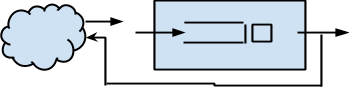
\includegraphics[width=262pt, height=67pt, keepaspectratio=true]{TP1-Colas-fig048.png}
%%%\caption{This should be the caption for \texttt{TP1-Colas-fig048.png}.}
%%%\end{figure}
%
%\vspace{13pt}
%%%\begin{figure}[htbp]
%\includegraphics[width=91pt, height=14pt, keepaspectratio=true]{TP1-Colas-fig049.png}
%%%\caption{This should be the caption for \texttt{TP1-Colas-fig049.png}.}
%%%\end{figure}
%
%\vspace{27pt}
%\begin{tabular}{|>{\raggedright}p{28pt}|>{\raggedright}p{26pt}|>{\raggedright}p{26pt}|>{\raggedright}p{26pt}|>{\raggedright}p{26pt}|>{\raggedright}p{26pt}|>{\raggedright}p{26pt}|>{\raggedright}p{26pt}|>{\raggedright}p{26pt}|}
%\hline
%n & P(n)
%\includegraphics[width=8pt, height=11pt, keepaspectratio=true]{TP1-Colas-fig050.png}
% & 
%\includegraphics[width=8pt, height=11pt, keepaspectratio=true]{TP1-Colas-fig051.png}
% &  & L & Lc & J & N' & H\tabularnewline
%\hline
%0 & P(0)
%\includegraphics[width=24pt, height=14pt, keepaspectratio=true]{TP1-Colas-fig052.png}
% &  & 0 & 0 & 0 & 4 & 4 & 0\tabularnewline
%\hline
%1 & P(1)
%\includegraphics[width=24pt, height=14pt, keepaspectratio=true]{TP1-Colas-fig053.png}
% & 
%\includegraphics[width=8pt, height=11pt, keepaspectratio=true]{TP1-Colas-fig054.png}
% &  & 1 & 0 & 3 & 4 & 1\tabularnewline
%\hline
%2 & P(2)
%\includegraphics[width=24pt, height=14pt, keepaspectratio=true]{TP1-Colas-fig055.png}
% & 
%\includegraphics[width=8pt, height=11pt, keepaspectratio=true]{TP1-Colas-fig056.png}
% &  & 2 & 1 & 2 & 4 & 1\tabularnewline
%\hline
%3 & P(3)
%\includegraphics[width=17pt, height=14pt, keepaspectratio=true]{TP1-Colas-fig057.png}
% & 
%\includegraphics[width=8pt, height=11pt, keepaspectratio=true]{TP1-Colas-fig058.png}
% &  & 3 & 2 & 1 & 4 & 1\tabularnewline
%\hline
%4 & P(4) & 0
%\includegraphics[width=8pt, height=11pt, keepaspectratio=true]{TP1-Colas-fig059.png}
% &  & 4 & 3 & 0 & 4 & 1\tabularnewline
%\hline
%.. & 0 & .. & .. & .. & .. & .. & .. & ..\tabularnewline
%\hline
%\end{tabular}
%
%\vspace{13pt}
%\leftskip=36pt
%\parindent=-18pt
%a.\tab 
%\includegraphics[width=199pt, height=14pt, keepaspectratio=true]{TP1-Colas-fig060.png}
%
%%%\begin{figure}[htbp]
%\includegraphics[width=158pt, height=29pt, keepaspectratio=true]{TP1-Colas-fig061.png}
%%%\caption{This should be the caption for \texttt{TP1-Colas-fig061.png}.}
%%%\end{figure}
%
%\vspace{13pt}
%%%\begin{figure}[htbp]
%\includegraphics[width=167pt, height=29pt, keepaspectratio=true]{TP1-Colas-fig062.png}
%%%\caption{This should be the caption for \texttt{TP1-Colas-fig062.png}.}
%%%\end{figure}
%
%\vspace{13pt}
%%%\begin{figure}[htbp]
%\includegraphics[width=170pt, height=29pt, keepaspectratio=true]{TP1-Colas-fig063.png}
%%%\caption{This should be the caption for \texttt{TP1-Colas-fig063.png}.}
%%%\end{figure}
%
%\vspace{13pt}
%%%\begin{figure}[htbp]
%\includegraphics[width=164pt, height=29pt, keepaspectratio=true]{TP1-Colas-fig064.png}
%%%\caption{This should be the caption for \texttt{TP1-Colas-fig064.png}.}
%%%\end{figure}
%
%\vspace{13pt}
%%%\begin{figure}[htbp]
%\includegraphics[width=155pt, height=32pt, keepaspectratio=true]{TP1-Colas-fig065.png}
%%%\caption{This should be the caption for \texttt{TP1-Colas-fig065.png}.}
%%%\end{figure}
%
%\vspace{13pt}
%%%\begin{figure}[htbp]
%\includegraphics[width=461pt, height=29pt, keepaspectratio=true]{TP1-Colas-fig066.png}
%%%\caption{This should be the caption for \texttt{TP1-Colas-fig066.png}.}
%%%\end{figure}
%
%\vspace{13pt}
%%%\begin{figure}[htbp]
%\includegraphics[width=59pt, height=11pt, keepaspectratio=true]{TP1-Colas-fig067.png}
%%%\caption{This should be the caption for \texttt{TP1-Colas-fig067.png}.}
%%%\end{figure}
%
%\vspace{13pt}
%{\large{}b.\tab }
%\includegraphics[width=77pt, height=14pt, keepaspectratio=true]{TP1-Colas-fig068.png}
%
%{\large{}c.\tab }
%\includegraphics[width=518pt, height=14pt, keepaspectratio=true]{TP1-Colas-fig069.png}
%
%\includegraphics[width=156pt, height=19pt, keepaspectratio=true]{TP1-Colas-fig070.png}
%
%d.\tab Para saber si conviene contratar un nuevo empleado a \$700 por mes, se plantea 
%un nuevo sistema con 2 canales: PPMN:\label{h.we0rz647mwgh}
%
%\vspace{21pt}
%\leftskip=0pt
%\parindent=0pt
%{\color{color01} \emph{Hipótesis}}
%
%\leftskip=36pt
%\parindent=-18pt
%\tab El proceso de llegada de los clientes responde a un proceso Poisson.
%
%\tab El proceso de atención de los clientes responde a un proceso Poisson.
%
%\tab La población es infinita
%
%\tab Se forma una única cola frente al canal de atención.
%
%\tab Existe un único canal de atención.
%
%\tab La capacidad del sistema es \emph{finita}
%
%\tab La atención de los clientes de la cola es FIFO
%
%\tab El sistema se encuentra en condiciones estables.
%
%\tab La población no presenta el fenómeno de impaciencia.\label{h.oy764fhdy6s9}
%
%\vspace{21pt}
%\leftskip=0pt
%\parindent=0pt
%{\color{color01} \emph{Modelo}}
%
%Este problema es un modelo de población finita:  PP1(N') con N'=4
%
%%%\begin{figure}[htbp]
%\includegraphics[width=262pt, height=67pt, keepaspectratio=true]{TP1-Colas-fig071.png}
%%%\caption{This should be the caption for \texttt{TP1-Colas-fig071.png}.}
%%%\end{figure}
%
%\vspace{13pt}
%%%\begin{figure}[htbp]
%\includegraphics[width=91pt, height=14pt, keepaspectratio=true]{TP1-Colas-fig072.png}
%%%\caption{This should be the caption for \texttt{TP1-Colas-fig072.png}.}
%%%\end{figure}
%
%\vspace{55pt}
%\begin{tabular}{|>{\raggedright}p{28pt}|>{\raggedright}p{26pt}|>{\raggedright}p{26pt}|>{\raggedright}p{26pt}|>{\raggedright}p{26pt}|>{\raggedright}p{26pt}|>{\raggedright}p{26pt}|>{\raggedright}p{26pt}|>{\raggedright}p{26pt}|}
%\hline
%n & P(n)
%\includegraphics[width=8pt, height=11pt, keepaspectratio=true]{TP1-Colas-fig073.png}
% & 
%\includegraphics[width=8pt, height=11pt, keepaspectratio=true]{TP1-Colas-fig074.png}
% &  & L & Lc & J & N' & H\tabularnewline
%\hline
%0 & P(0)
%\includegraphics[width=24pt, height=14pt, keepaspectratio=true]{TP1-Colas-fig075.png}
% & 8
%\includegraphics[width=24pt, height=14pt, keepaspectratio=true]{TP1-Colas-fig076.wmf}
% & 0 & 0 & 0 & 4 & 4 & 0\tabularnewline
%\hline
%1 & P(1)
%\includegraphics[width=24pt, height=14pt, keepaspectratio=true]{TP1-Colas-fig077.png}
% & 8
%\includegraphics[width=24pt, height=14pt, keepaspectratio=true]{TP1-Colas-fig078.wmf}
%
%\includegraphics[width=8pt, height=11pt, keepaspectratio=true]{TP1-Colas-fig079.png}
% &  & 1 & 0 & 3 & 4 & 1\tabularnewline
%\hline
%2 & P(2)
%\includegraphics[width=24pt, height=14pt, keepaspectratio=true]{TP1-Colas-fig080.png}
% & 8
%\includegraphics[width=24pt, height=14pt, keepaspectratio=true]{TP1-Colas-fig081.wmf}
%
%\includegraphics[width=15pt, height=14pt, keepaspectratio=true]{TP1-Colas-fig082.png}
% &  & 2 & 1 & 2 & 4 & 1\tabularnewline
%\hline
%3 & P(3)
%\includegraphics[width=17pt, height=14pt, keepaspectratio=true]{TP1-Colas-fig083.png}
% & 8
%\includegraphics[width=17pt, height=14pt, keepaspectratio=true]{TP1-Colas-fig084.wmf}
%
%\includegraphics[width=15pt, height=14pt, keepaspectratio=true]{TP1-Colas-fig085.png}
% &  & 3 & 2 & 1 & 4 & 1\tabularnewline
%\hline
%4 & P(4) & 0
%\includegraphics[width=15pt, height=14pt, keepaspectratio=true]{TP1-Colas-fig086.png}
% &  & 4 & 3 & 0 & 4 & 1\tabularnewline
%\hline
%.. & 0 & .. & .. & .. & .. & .. & .. & ..\tabularnewline
%\hline
%\end{tabular}
%
%\vspace{27pt}
%%%\begin{figure}[htbp]
%\includegraphics[width=199pt, height=14pt, keepaspectratio=true]{TP1-Colas-fig087.png}
%%%\caption{This should be the caption for \texttt{TP1-Colas-fig087.png}.}
%%%\end{figure}
%
%\vspace{13pt}
%%%\begin{figure}[htbp]
%\includegraphics[width=158pt, height=29pt, keepaspectratio=true]{TP1-Colas-fig088.png}
%%%\caption{This should be the caption for \texttt{TP1-Colas-fig088.png}.}
%%%\end{figure}
%
%\vspace{13pt}
%%%\begin{figure}[htbp]
%\includegraphics[width=161pt, height=31pt, keepaspectratio=true]{TP1-Colas-fig089.png}
%%%\caption{This should be the caption for \texttt{TP1-Colas-fig089.png}.}
%%%\end{figure}
%
%\vspace{13pt}
%%%\begin{figure}[htbp]
%\includegraphics[width=162pt, height=31pt, keepaspectratio=true]{TP1-Colas-fig090.png}
%%%\caption{This should be the caption for \texttt{TP1-Colas-fig090.png}.}
%%%\end{figure}
%
%\vspace{13pt}
%%%\begin{figure}[htbp]
%\includegraphics[width=156pt, height=31pt, keepaspectratio=true]{TP1-Colas-fig091.png}
%%%\caption{This should be the caption for \texttt{TP1-Colas-fig091.png}.}
%%%\end{figure}
%
%\vspace{13pt}
%%%\begin{figure}[htbp]
%\includegraphics[width=155pt, height=32pt, keepaspectratio=true]{TP1-Colas-fig092.png}
%%%\caption{This should be the caption for \texttt{TP1-Colas-fig092.png}.}
%%%\end{figure}
%
%\vspace{13pt}
%%%\begin{figure}[htbp]
%\includegraphics[width=446pt, height=29pt, keepaspectratio=true]{TP1-Colas-fig093.png}
%%%\caption{This should be the caption for \texttt{TP1-Colas-fig093.png}.}
%%%\end{figure}
%
%\vspace{13pt}
%%%\begin{figure}[htbp]
%\includegraphics[width=60pt, height=14pt, keepaspectratio=true]{TP1-Colas-fig094.png}
%%%\caption{This should be the caption for \texttt{TP1-Colas-fig094.png}.}
%%%\end{figure}
%
%\vspace{27pt}
%%%\begin{figure}[htbp]
%\includegraphics[width=140pt, height=14pt, keepaspectratio=true]{TP1-Colas-fig095.png}
%%%\caption{This should be the caption for \texttt{TP1-Colas-fig095.png}.}
%%%\end{figure}
%
%8
%\includegraphics[width=140pt, height=14pt, keepaspectratio=true]{TP1-Colas-fig096.wmf}
%
%{\large{}Antes:}
%
%%%\begin{figure}[htbp]
%\includegraphics[width=458pt, height=15pt, keepaspectratio=true]{TP1-Colas-fig097.png}
%%%\caption{This should be the caption for \texttt{TP1-Colas-fig097.png}.}
%%%\end{figure}
%
%\vspace{13pt}
%{\large{}Ahora:}
%
%%%\begin{figure}[htbp]
%\includegraphics[width=461pt, height=15pt, keepaspectratio=true]{TP1-Colas-fig098.png}
%%%\caption{This should be the caption for \texttt{TP1-Colas-fig098.png}.}
%%%\end{figure}
%
%\vspace{27pt}
%%%\begin{figure}[htbp]
%\includegraphics[width=344pt, height=14pt, keepaspectratio=true]{TP1-Colas-fig099.png}
%%%\caption{This should be the caption for \texttt{TP1-Colas-fig099.png}.}
%%%\end{figure}
%
%8
%\includegraphics[width=344pt, height=14pt, keepaspectratio=true]{TP1-Colas-fig100.wmf}
%
%\newpage
%
\part{Apéndice}
\appendix

\section{Enunciado original}\label{sec:enunciado}
\includepdf[pages={-}]{enunciado.pdf}

\clearpage
\end{document}
